\subsection{Einführung von Bloch-Diagrammen}
\subsubsection*{Selbstenergie-Blöcke und Dyson-Gleichung}

\stp{In der Mehrheit der quantenstatistischen Probleme ist es nicht möglich, sich auf die ersten Terme der Störungsreihe zu beschränken.}

\stp{Selbstenergie-Blöcke: Betrachten alle Diagramme, die nicht aus zwei oder mehreren Teilen bestehen, die nur durch eine $G$-Linie verbunden sind.}\\
$\hookrightarrow$ z.B. beide Diagramme in 1. Ordnung und $e-j$ in 2. Ordnung

\stp{Diese inneren Anteile haben folgende Struktur:}
\begin{figure}[ht]
  \centering
  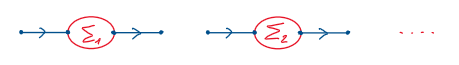
\includegraphics[width=0.5\textwidth]{temp_diagrams/11_05_diagrams/img1_modules.png}
  \label{fig:Selbstenergie_Block}
\end{figure}
\stp{Die Summe aller Selbstenergie-Blöcke ist die Selbstenergie:}
\begin{equation}
  \Sigma(1,2) = \sum\limits_i \Sigma_i(1,2)
\end{equation}
\stp{Die Gesamtheit aller Diagramme lässt sich darstellen als:}
\begin{figure}[ht]
  \centering
  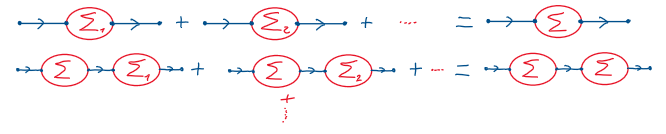
\includegraphics[width=0.6\textwidth]{temp_diagrams/11_05_diagrams/img2_comb_modules.png}
  \label{fig:Selbstenergie_Bloecke}
\end{figure}
\begin{equation}
  \begin{aligned}
    G & = G_0 + G_0 \Sigma(G_0 + G_0 \Sigma G_0 + G_0 \Sigma G_0 \Sigma G_0 + \ldots) \\
      & = G_0 + G_0 \Sigma G
  \end{aligned}
\end{equation}
\stp{Mit Argumenten und Integral über innere Punkte ergibt sich die \textbf{Dyson-Gleichung}:}
\begin{equation}
  \boxed{G(1,2) = G_0(1,2) + \int d3 \, d4 \, G_0(1,3) \Sigma(3,4) G(4,2)}
\end{equation}
\begin{figure}[ht]
  \centering
  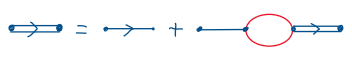
\includegraphics[width=0.4\textwidth]{temp_diagrams/11_05_diagrams/img3_dyson.png}
  \label{fig:Dyson_Gleichung}
\end{figure}
$\Rightarrow$ die rekursive Lösung der Dyson-Gleichung generiert die gesamte Störungsreihe.

\subsubsection*{Polarisationsblöcke}

\stp{Ähnliche Analyse kann für die WW durchgeführt werden:}
Coulomb WW in niedriger Ordnung wird in Diagrammen höherer Ordnung ersetzt durch zwei Coulomb-Linien mit Einschlüssen.
\begin{figure}[ht]
  \centering
  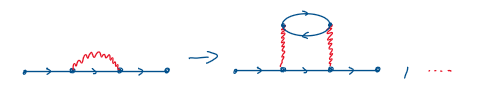
\includegraphics[width=0.55\textwidth]{temp_diagrams/11_05_diagrams/img4_int_progress.png}
  \label{fig:int_progress}
\end{figure}
\begin{figure}[ht]
  \centering
  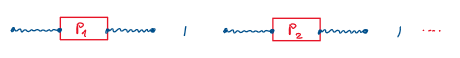
\includegraphics[width=0.55\textwidth]{temp_diagrams/11_05_diagrams/img5_int_modules.png}
  \label{fig:int_modules}
\end{figure}
\stp{Definition:}
Die Diagramme, die nicht aus zwei Teilen bestehen, die nur durch eine $v$-Linie verbunden sind \\
$\rightarrow$ die Einschlüsse zwischen zwei Coulomb-Linien sind die \textbf{Polarisationsblöcke}.

\stp{Summe aller Polarisationsblöcke:}
\begin{equation}
  P(\eta) = \sum\limits_i P_i(\eta)
\end{equation}

Durch eine analoge Argumentation wie bei der Selbstenergie erhält man:
\begin{equation}
  \begin{aligned}
    W & = V + VPV + VPVPV + \ldots \\
      & = V + VP(V + VPV)          \\
      & = V + VPW
  \end{aligned}
\end{equation}
\stp{Mit Argumenten und Integrationsvariablen ergibt sich die Dyson-Gleichung für die abgeschirmte WW:}
\begin{equation}
  \boxed{W(1,2) = V(1,2) + \int d3 \, d4 \, u(1,3) P(3,4) W(4,2)}
\end{equation}
Dies ist die \textbf{Bethe-Salpeter-Gleichung für abgeschirmte Coulomb-Wechselwirkung} (Dyson-Gleichung für $W$ statt $U$).

\lend{Vorl. 11.05.2026}[Vorl. 18.05.2026]

\subsubsection*{Vertexblöcke}
Vertexblöcke sind alle irreduziblen Diagrammteile mit genau drei Eckpunkten. Dabei entspricht eine der drei angeschlossenen Linien einer Coulomb-Wechselwirkung $v$, die beiden anderen sind freie Propagatorlinien $G_0$. Solche Blöcke beschreiben also die elementare Kopplung einer WW-Linie an zwei Fermionenlinien.
\begin{figure}[ht]
  \centering
  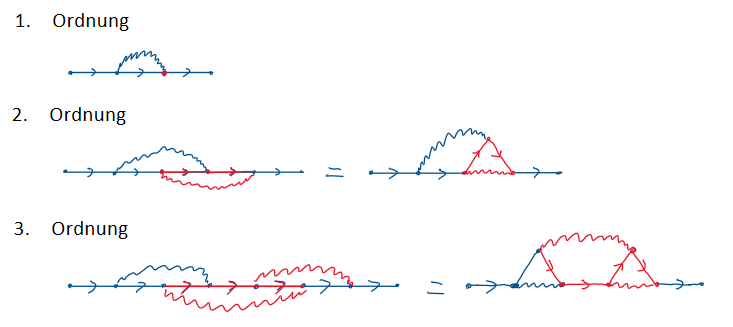
\includegraphics[width=0.75\textwidth]{temp_diagrams/18_05_diagrams/vertexParts.png}
  \label{fig:vertexParts}
\end{figure}\pagebreak
Vertexblöcke werden oft auch mit $\Gamma$ bezeichnet.

\subsubsection*{Aufwertung: Methode zur Bestimmung von $$\Sigma$$ und $$P$$ }
Alle Selbstenergie und Polarisationsdiagramme lassen sich durch Aufwertung der Diagramme niedrigster Ordnung erstellen (wie man sich zeichnerisch vergewissern kann)\\
$\hookrightarrow$ Mit Aufwertung lassen sich alle erstellen, selbstenergie muss man dann raussuchen

\begin{enumerate}
  \item $G_0 \Rightarrow G$ in bisherige $G_0$-Linien alle möglichen Selbstenergie \textbf{beiträge} einschieben
  \item $V \Rightarrow V_s$ in v-Linien alle möglichen Polarisationsblöcke
  \item Einfügen der Vertexbeiträge
\end{enumerate}

\underline{Selbstenergie:}\\
Die Komplette selbstenergie entsteht durch Aufwertung der beiden niedrigsten Selbstenergie-Diagramme
\begin{figure}[ht]
  \centering
  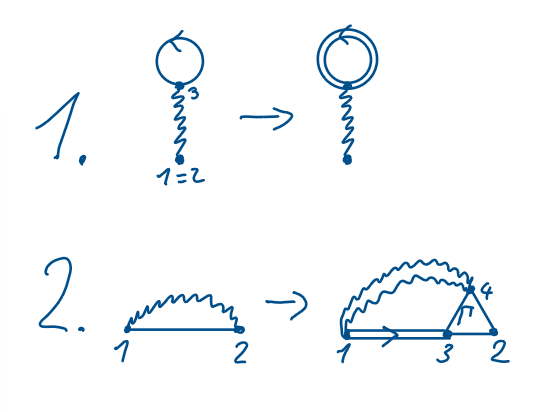
\includegraphics[width=0.4\textwidth]{temp_diagrams/18_05_diagrams/auf_selbstenergie.png}
  \label{fig:auf_selbstenergie}
\end{figure}
Zu 1: man kann sich zeichnerisch davon überzeuge, dass die v-Linie nicht aufgewertet werden darf. Hierdurch würden Beiträge entstehen, die bereits bei $G_0$ Aufwertung geliefert werden.

\underline{Polarisations-blöcke:}\\
Die komplette polarisationsfunktion entsteht durch die Aufwertung des Polarisationsblocks niedrigster Ordnung
\begin{figure}[H]
  \centering
  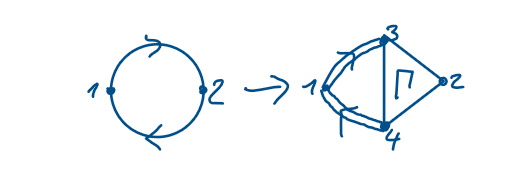
\includegraphics[width=0.4\textwidth]{temp_diagrams/18_05_diagrams/auf_polaristation.png}
  \label{fig:auf_pol}
\end{figure}

\subsubsection*{Zusammenfassung der analytischen Ausdrücke}
\begin{equation}
  \begin{aligned}
    \Sigma(1,2) &= -i\hbar \int d3 \, v(1-2) \, G(3,3^+) \\
                &\quad + i\hbar \int d3 \, d4 \, G(1,3) \, v(1,4) \, \Gamma(3,4,2)
  \end{aligned}
\end{equation}

\begin{equation}
  P(1,2) = i\hbar \int d3 \, d4 \, G(1,3) \, G(4,1) \, \Gamma(3,2,4)
\end{equation}

\noindent niedrigste Näherung für $\Gamma$:
\begin{equation}
  \Gamma_0(1,2,3) = \delta(1-2) \, \delta(1-3)
\end{equation}
